\documentclass[tikz,border=1cm]{standalone}
\usetikzlibrary{spy}
\usepackage{tkz-euclide}
\usepackage{amsmath}
\newcommand*\mydrawellipse[4][]{%
% #2=pointA;#3==pointB;#4= ratio of y on x
    \tkzCalcLength(#2,#3)%
    \tkzGetLength{tmpdistance}%
    \tkzFindSlopeAngle(#2,#3) %
    \tkzGetAngle{tmpangle}%
    \begin{scope}[rotate=\tmpangle]
    \draw[thick,#1] (#3) arc [start angle=0,delta angle=180,x radius=\fpeval{\tmpdistance/2} cm,y radius=\fpeval{\tmpdistance * (#4) / 2}cm] (#2);
    \draw[thick,#1] (#2) arc[start angle=180,delta angle=180,x radius=\fpeval{\tmpdistance/2} cm,y radius=\fpeval{\tmpdistance * (#4) / 2}cm] (#3);
    \end{scope}
}
\begin{document}
\tikzset{%
    every picture/.style={
            spy using outlines={%
                circle,size=4cm,
                magnification=3,
                connect spies,
            }
        }
}%
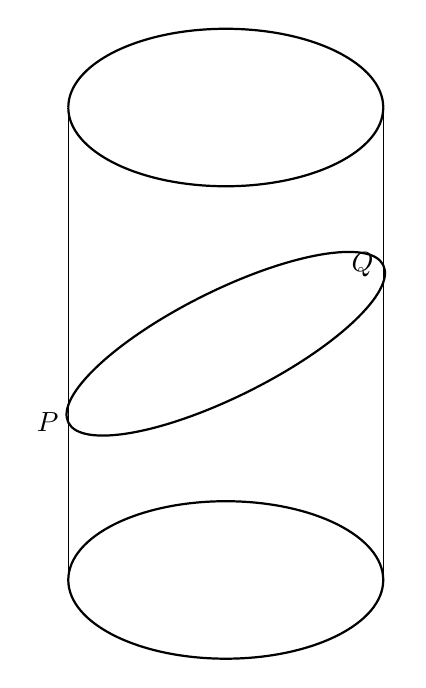
\begin{tikzpicture}
\tkzDefPoints{2/0/A,-2/0/B,2/6/C,-2/6/D}
\tkzDrawSegments(A,C B,D)
\mydrawellipse{A}{B}{0.5}
\mydrawellipse{C}{D}{0.5}
\tkzDefPoints{-2/2/P,2/4/Q}
\tkzLabelPoints[left](P,Q)
\mydrawellipse{P}{Q}{0.3}
\spy[red] on (P) in node [left] at (-3,4);
\spy[blue] on (Q) in node [right] at (4,3);
\end{tikzpicture}
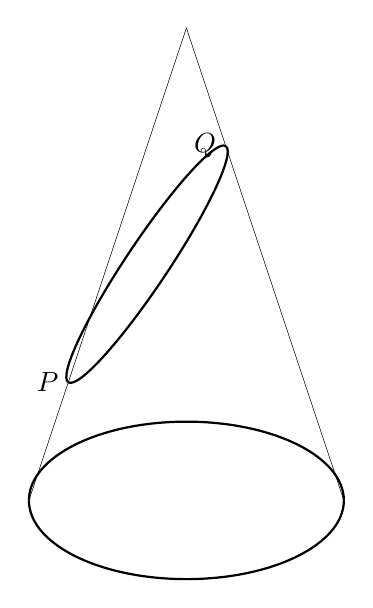
\begin{tikzpicture}
    \tkzDefPoints{2/0/A,-2/0/B,0/6/C}
    \tkzDrawSegments(A,C B,C)
    \mydrawellipse{A}{B}{0.5}
    \tkzDefPoints{-1.5/1.5/P,.5/4.5/Q}
    \tkzLabelPoints[left](P,Q)
    \mydrawellipse{P}{Q}{0.15}
    \spy[red] on (P) in node [left] at (-3,4);
    \spy[blue] on (Q) in node [right] at (4,3);
    \spy[red] on (B) in node [left] at (-3,-2);
    \spy[blue] on (A) in node [right] at (4,-1.5);
\end{tikzpicture}
\end{document}